\documentclass[]{article}
\usepackage{lmodern}
\usepackage{amssymb,amsmath}
\usepackage{ifxetex,ifluatex}
\usepackage{fixltx2e} % provides \textsubscript
\ifnum 0\ifxetex 1\fi\ifluatex 1\fi=0 % if pdftex
  \usepackage[T1]{fontenc}
  \usepackage[utf8]{inputenc}
\else % if luatex or xelatex
  \ifxetex
    \usepackage{mathspec}
  \else
    \usepackage{fontspec}
  \fi
  \defaultfontfeatures{Ligatures=TeX,Scale=MatchLowercase}
\fi
% use upquote if available, for straight quotes in verbatim environments
\IfFileExists{upquote.sty}{\usepackage{upquote}}{}
% use microtype if available
\IfFileExists{microtype.sty}{%
\usepackage{microtype}
\UseMicrotypeSet[protrusion]{basicmath} % disable protrusion for tt fonts
}{}
\usepackage[margin=1in]{geometry}
\usepackage{hyperref}
\hypersetup{unicode=true,
            pdfborder={0 0 0},
            breaklinks=true}
\urlstyle{same}  % don't use monospace font for urls
\usepackage{color}
\usepackage{fancyvrb}
\newcommand{\VerbBar}{|}
\newcommand{\VERB}{\Verb[commandchars=\\\{\}]}
\DefineVerbatimEnvironment{Highlighting}{Verbatim}{commandchars=\\\{\}}
% Add ',fontsize=\small' for more characters per line
\usepackage{framed}
\definecolor{shadecolor}{RGB}{248,248,248}
\newenvironment{Shaded}{\begin{snugshade}}{\end{snugshade}}
\newcommand{\KeywordTok}[1]{\textcolor[rgb]{0.13,0.29,0.53}{\textbf{#1}}}
\newcommand{\DataTypeTok}[1]{\textcolor[rgb]{0.13,0.29,0.53}{#1}}
\newcommand{\DecValTok}[1]{\textcolor[rgb]{0.00,0.00,0.81}{#1}}
\newcommand{\BaseNTok}[1]{\textcolor[rgb]{0.00,0.00,0.81}{#1}}
\newcommand{\FloatTok}[1]{\textcolor[rgb]{0.00,0.00,0.81}{#1}}
\newcommand{\ConstantTok}[1]{\textcolor[rgb]{0.00,0.00,0.00}{#1}}
\newcommand{\CharTok}[1]{\textcolor[rgb]{0.31,0.60,0.02}{#1}}
\newcommand{\SpecialCharTok}[1]{\textcolor[rgb]{0.00,0.00,0.00}{#1}}
\newcommand{\StringTok}[1]{\textcolor[rgb]{0.31,0.60,0.02}{#1}}
\newcommand{\VerbatimStringTok}[1]{\textcolor[rgb]{0.31,0.60,0.02}{#1}}
\newcommand{\SpecialStringTok}[1]{\textcolor[rgb]{0.31,0.60,0.02}{#1}}
\newcommand{\ImportTok}[1]{#1}
\newcommand{\CommentTok}[1]{\textcolor[rgb]{0.56,0.35,0.01}{\textit{#1}}}
\newcommand{\DocumentationTok}[1]{\textcolor[rgb]{0.56,0.35,0.01}{\textbf{\textit{#1}}}}
\newcommand{\AnnotationTok}[1]{\textcolor[rgb]{0.56,0.35,0.01}{\textbf{\textit{#1}}}}
\newcommand{\CommentVarTok}[1]{\textcolor[rgb]{0.56,0.35,0.01}{\textbf{\textit{#1}}}}
\newcommand{\OtherTok}[1]{\textcolor[rgb]{0.56,0.35,0.01}{#1}}
\newcommand{\FunctionTok}[1]{\textcolor[rgb]{0.00,0.00,0.00}{#1}}
\newcommand{\VariableTok}[1]{\textcolor[rgb]{0.00,0.00,0.00}{#1}}
\newcommand{\ControlFlowTok}[1]{\textcolor[rgb]{0.13,0.29,0.53}{\textbf{#1}}}
\newcommand{\OperatorTok}[1]{\textcolor[rgb]{0.81,0.36,0.00}{\textbf{#1}}}
\newcommand{\BuiltInTok}[1]{#1}
\newcommand{\ExtensionTok}[1]{#1}
\newcommand{\PreprocessorTok}[1]{\textcolor[rgb]{0.56,0.35,0.01}{\textit{#1}}}
\newcommand{\AttributeTok}[1]{\textcolor[rgb]{0.77,0.63,0.00}{#1}}
\newcommand{\RegionMarkerTok}[1]{#1}
\newcommand{\InformationTok}[1]{\textcolor[rgb]{0.56,0.35,0.01}{\textbf{\textit{#1}}}}
\newcommand{\WarningTok}[1]{\textcolor[rgb]{0.56,0.35,0.01}{\textbf{\textit{#1}}}}
\newcommand{\AlertTok}[1]{\textcolor[rgb]{0.94,0.16,0.16}{#1}}
\newcommand{\ErrorTok}[1]{\textcolor[rgb]{0.64,0.00,0.00}{\textbf{#1}}}
\newcommand{\NormalTok}[1]{#1}
\usepackage{graphicx,grffile}
\makeatletter
\def\maxwidth{\ifdim\Gin@nat@width>\linewidth\linewidth\else\Gin@nat@width\fi}
\def\maxheight{\ifdim\Gin@nat@height>\textheight\textheight\else\Gin@nat@height\fi}
\makeatother
% Scale images if necessary, so that they will not overflow the page
% margins by default, and it is still possible to overwrite the defaults
% using explicit options in \includegraphics[width, height, ...]{}
\setkeys{Gin}{width=\maxwidth,height=\maxheight,keepaspectratio}
\IfFileExists{parskip.sty}{%
\usepackage{parskip}
}{% else
\setlength{\parindent}{0pt}
\setlength{\parskip}{6pt plus 2pt minus 1pt}
}
\setlength{\emergencystretch}{3em}  % prevent overfull lines
\providecommand{\tightlist}{%
  \setlength{\itemsep}{0pt}\setlength{\parskip}{0pt}}
\setcounter{secnumdepth}{0}
% Redefines (sub)paragraphs to behave more like sections
\ifx\paragraph\undefined\else
\let\oldparagraph\paragraph
\renewcommand{\paragraph}[1]{\oldparagraph{#1}\mbox{}}
\fi
\ifx\subparagraph\undefined\else
\let\oldsubparagraph\subparagraph
\renewcommand{\subparagraph}[1]{\oldsubparagraph{#1}\mbox{}}
\fi

%%% Use protect on footnotes to avoid problems with footnotes in titles
\let\rmarkdownfootnote\footnote%
\def\footnote{\protect\rmarkdownfootnote}

%%% Change title format to be more compact
\usepackage{titling}

% Create subtitle command for use in maketitle
\newcommand{\subtitle}[1]{
  \posttitle{
    \begin{center}\large#1\end{center}
    }
}

\setlength{\droptitle}{-2em}

  \title{}
    \pretitle{\vspace{\droptitle}}
  \posttitle{}
    \author{}
    \preauthor{}\postauthor{}
    \date{}
    \predate{}\postdate{}
  
\usepackage{float}

\begin{document}

\begin{centering}

\vspace*{5 cm}

\Huge

{\bf Procesamiento de datos}

\vspace{3 cm}

\Large
Marco Andrés Vázquez Hernández

\vspace{1 cm}
\normalsize
Práctica 1. 

Septiembre de 2018

\normalsize
Instituto Politécnico Nacional


\end{centering}

\newpage

\section{Descripción}\label{descripcion}

Instrucciones

\begin{enumerate}
\def\labelenumi{\arabic{enumi}.}
\tightlist
\item
  Integrar los cuatro archivos en una tabla llamada statusVehiculo
\item
  Trasformar los datos a distancia recorrida y combustible utilizado de
  cada vehículo por DIA, utilizando los siguientes diagnósticos
\end{enumerate}

\begin{enumerate}
\def\labelenumi{\alph{enumi}.}
\item
\begin{verbatim}
'DiagnosticTotalFuelUsedId'
\end{verbatim}
\item
\begin{verbatim}
'DiagnosticOdometerId'
\end{verbatim}
\end{enumerate}

\begin{enumerate}
\def\labelenumi{\arabic{enumi}.}
\setcounter{enumi}{2}
\tightlist
\item
  Graficar la relación entre distancia y combustible diario.
\item
  Sacar el modelo de regresión lineal y = a*x + b
\item
  Predecir los valores con ruido o sucios con el modelo anterior
\item
  Contestar lo siguiente:
\end{enumerate}

\begin{enumerate}
\def\labelenumi{\alph{enumi}.}
\item
\begin{verbatim}
¿Qué vehículo da mayor rendimiento?
\end{verbatim}
\item
\begin{verbatim}
¿Qué vehículo trabajó mas días?
\end{verbatim}
\item
\begin{verbatim}
¿Cuál es el combustible total utilizado por la flota por semana?
\end{verbatim}
\item
\begin{verbatim}
¿Cuál es la correlación entre ambas variables (distancia, combustible)?
\end{verbatim}
\end{enumerate}

\begin{enumerate}
\def\labelenumi{\arabic{enumi}.}
\setcounter{enumi}{6}
\tightlist
\item
  Documentar los resultados
\end{enumerate}

Para la elaboración de la práctica se utilizó la herramienta R Studio.

\section{Integración de los archivos}\label{integracion-de-los-archivos}

Se cargaron los datos desde los archivos .csv y se unieron por filas
para crear una tabla con las clumnas
``vehiculo'',``fecha'',``diagnostico'' y ``valor''.

\begin{Shaded}
\begin{Highlighting}[]
\NormalTok{wd<-}\StringTok{"C:/Users/marco/IPN_BigData/Modulo2/Práctica 1"}
\KeywordTok{setwd}\NormalTok{(wd)}
\KeywordTok{library}\NormalTok{(reshape2)}
\NormalTok{data1<-}\KeywordTok{read.csv}\NormalTok{(}\StringTok{"StatusData.csv"}\NormalTok{, }\DataTypeTok{header=}\NormalTok{F)}
\NormalTok{data2<-}\KeywordTok{read.csv}\NormalTok{(}\StringTok{"StatusData2.csv"}\NormalTok{, }\DataTypeTok{header=}\NormalTok{F)}
\NormalTok{data3<-}\KeywordTok{read.csv}\NormalTok{(}\StringTok{"StatusData3.csv"}\NormalTok{, }\DataTypeTok{header=}\NormalTok{F)}
\NormalTok{data4<-}\KeywordTok{read.csv}\NormalTok{(}\StringTok{"StatusData4.csv"}\NormalTok{, }\DataTypeTok{header=}\NormalTok{F)}
\NormalTok{data<-}\KeywordTok{rbind}\NormalTok{(data1,data2,data3,data4)}
\KeywordTok{colnames}\NormalTok{(data)<-}\KeywordTok{c}\NormalTok{(}\StringTok{"vehiculo"}\NormalTok{,}\StringTok{"fecha"}\NormalTok{,}\StringTok{"diagnostico"}\NormalTok{,}\StringTok{"valor"}\NormalTok{)}
\end{Highlighting}
\end{Shaded}

\section{Transformación de datos.}\label{transformacion-de-datos.}

\subsection{Limpiado de datos.}\label{limpiado-de-datos.}

Primero se filtraron los datos para incluir solo las variables
``DiagnosticTotalFuelUsedId'' y ``DiagnosticOdometerId''; se crearon
fechas adicionales con los formatos adecuados y se separaron los datos
en dos tablas (para cada variable).

\begin{Shaded}
\begin{Highlighting}[]
\NormalTok{tidy<-data[data}\OperatorTok{$}\NormalTok{diagnostico }\OperatorTok\StringTok{ }\KeywordTok{c}\NormalTok{(}\StringTok{"DiagnosticTotalFuelUsedId"}\NormalTok{,}\StringTok{"DiagnosticOdometerId"}\NormalTok{),]}
\NormalTok{tidy<-tidy[}\OperatorTok{!}\KeywordTok{duplicated}\NormalTok{(tidy),]}

\NormalTok{tidy}\OperatorTok{$}\NormalTok{fecha2<-}\KeywordTok{gsub}\NormalTok{(}\StringTok{"T"}\NormalTok{,}\StringTok{" "}\NormalTok{, tidy}\OperatorTok{$}\NormalTok{fecha)}
\NormalTok{tidy}\OperatorTok{$}\NormalTok{fecha2<-}\KeywordTok{gsub}\NormalTok{(}\StringTok{"Z"}\NormalTok{,}\StringTok{""}\NormalTok{, tidy}\OperatorTok{$}\NormalTok{fecha2)}
\NormalTok{tidy}\OperatorTok{$}\NormalTok{fecha2<-}\KeywordTok{as.POSIXct}\NormalTok{(tidy}\OperatorTok{$}\NormalTok{fecha2)}
\NormalTok{tidy}\OperatorTok{$}\NormalTok{fecha3<-}\KeywordTok{as.Date}\NormalTok{(tidy}\OperatorTok{$}\NormalTok{fecha2)}

\NormalTok{odom<-tidy[tidy}\OperatorTok{$}\NormalTok{diagnostico}\OperatorTok{==}\StringTok{"DiagnosticOdometerId"}\NormalTok{,]}
\NormalTok{fuel<-tidy[tidy}\OperatorTok{$}\NormalTok{diagnostico}\OperatorTok{==}\StringTok{"DiagnosticTotalFuelUsedId"}\NormalTok{,]}
\end{Highlighting}
\end{Shaded}

\subsection{Agrupación por día.}\label{agrupacion-por-dia.}

Se agruparon los datos por día tomando el valor mínimo del día.

\begin{Shaded}
\begin{Highlighting}[]
\NormalTok{aggodom<-}\KeywordTok{aggregate}\NormalTok{(odom}\OperatorTok{$}\NormalTok{valor, }\DataTypeTok{by=}\KeywordTok{list}\NormalTok{(odom}\OperatorTok{$}\NormalTok{vehiculo, odom}\OperatorTok{$}\NormalTok{fecha3), min)}
\KeywordTok{colnames}\NormalTok{(aggodom)<-}\KeywordTok{c}\NormalTok{(}\StringTok{"vehiculo"}\NormalTok{,}\StringTok{"fecha3"}\NormalTok{,}\StringTok{"odom"}\NormalTok{)}
\NormalTok{aggfuel<-}\KeywordTok{aggregate}\NormalTok{(fuel}\OperatorTok{$}\NormalTok{valor, }\DataTypeTok{by=}\KeywordTok{list}\NormalTok{(fuel}\OperatorTok{$}\NormalTok{vehiculo, fuel}\OperatorTok{$}\NormalTok{fecha3),min)}
\KeywordTok{colnames}\NormalTok{(aggfuel)<-}\KeywordTok{c}\NormalTok{(}\StringTok{"vehiculo"}\NormalTok{,}\StringTok{"fecha3"}\NormalTok{,}\StringTok{"fuel"}\NormalTok{)}
\end{Highlighting}
\end{Shaded}

\subsection{Normalización de valores por lag
diff.}\label{normalizacion-de-valores-por-lag-diff.}

Debido a que los odómetros y la cantidad acumulada de combustible de
cada vehículo puede variar de acuerdo a la antiguedad del vehículo, se
hizo una normalización por medio de considerar las diferencias entre
cada día. En otras palabras, para cada vehículo se ajustó el valor para
que en vez de tomar en cuenta el acumulado se tomara la distancia
recorrida y lo que consumió de gasolina únicamente en ese día.

Esto hace que el primer día ambos valores; distancia y combustible sean
cero. Es decir, debido a que no se tienen los datos del día anterior el
primer día se considera el ``inicio'' y por tanto sus valores serán 0 en
ambos casos.

\begin{Shaded}
\begin{Highlighting}[]
\CommentTok{# Normalización de valores por lag diff}

\ControlFlowTok{for}\NormalTok{ (v }\ControlFlowTok{in} \KeywordTok{unique}\NormalTok{(aggodom}\OperatorTok{$}\NormalTok{vehiculo))\{}
\NormalTok{  aux2<-aggodom[aggodom}\OperatorTok{$}\NormalTok{vehiculo}\OperatorTok{==}\NormalTok{v,]}
\NormalTok{  aux2<-aux2[}\KeywordTok{order}\NormalTok{(aux2}\OperatorTok{$}\NormalTok{fecha3),]}
\NormalTok{  aux2}\OperatorTok{$}\NormalTok{odomdif<-}\KeywordTok{c}\NormalTok{(}\DecValTok{0}\NormalTok{,}\KeywordTok{diff}\NormalTok{(aux2}\OperatorTok{$}\NormalTok{odom))}
  \ControlFlowTok{if}\NormalTok{(v }\OperatorTok{==}\StringTok{ "A1"}\NormalTok{)\{}
\NormalTok{    aux3<-aux2}
\NormalTok{  \} }\ControlFlowTok{else}\NormalTok{ \{}
\NormalTok{    aux3 <-}\StringTok{ }\KeywordTok{rbind}\NormalTok{(aux3,aux2)}
\NormalTok{  \}}
\NormalTok{\}}
\NormalTok{aggodom2<-aux3}
\NormalTok{aux3<-}\OtherTok{NULL}

\ControlFlowTok{for}\NormalTok{ (v }\ControlFlowTok{in} \KeywordTok{unique}\NormalTok{(aggfuel}\OperatorTok{$}\NormalTok{vehiculo))\{}
\NormalTok{  aux2<-aggfuel[aggfuel}\OperatorTok{$}\NormalTok{vehiculo}\OperatorTok{==}\NormalTok{v,]}
\NormalTok{  aux2<-aux2[}\KeywordTok{order}\NormalTok{(aux2}\OperatorTok{$}\NormalTok{fecha3),]}
\NormalTok{  aux2}\OperatorTok{$}\NormalTok{fueldif<-}\KeywordTok{c}\NormalTok{(}\DecValTok{0}\NormalTok{,}\KeywordTok{diff}\NormalTok{(aux2}\OperatorTok{$}\NormalTok{fuel))}
  \ControlFlowTok{if}\NormalTok{(v }\OperatorTok{==}\StringTok{ "A1"}\NormalTok{)\{}
\NormalTok{    aux3<-aux2}
\NormalTok{  \} }\ControlFlowTok{else}\NormalTok{ \{}
\NormalTok{    aux3 <-}\StringTok{ }\KeywordTok{rbind}\NormalTok{(aux3,aux2)}
\NormalTok{  \}}
\NormalTok{\}}
\NormalTok{aggfuel2<-aux3}
\NormalTok{aux3<-}\OtherTok{NULL}
\end{Highlighting}
\end{Shaded}

\subsection{Unión de tablas.}\label{union-de-tablas.}

Finalmente se unieron ambas tablas por vehículo y fecha y se calcula la
variable de rendimiento.

\begin{Shaded}
\begin{Highlighting}[]
\NormalTok{dataf<-aggodom2}
\KeywordTok{colnames}\NormalTok{(dataf)<-}\KeywordTok{c}\NormalTok{(}\StringTok{"vehiculo"}\NormalTok{,}\StringTok{"fecha3"}\NormalTok{,}\StringTok{"odom"}\NormalTok{,}\StringTok{"odomdif"}\NormalTok{)}
\KeywordTok{colnames}\NormalTok{(aggfuel2)<-}\KeywordTok{c}\NormalTok{(}\StringTok{"vehiculo"}\NormalTok{,}\StringTok{"fecha3"}\NormalTok{,}\StringTok{"fuel"}\NormalTok{,}\StringTok{"fueldif"}\NormalTok{)}
\NormalTok{dataf<-}\KeywordTok{merge}\NormalTok{(dataf, aggfuel2, }\DataTypeTok{by=}\KeywordTok{c}\NormalTok{(}\StringTok{"vehiculo"}\NormalTok{,}\StringTok{"fecha3"}\NormalTok{), }\DataTypeTok{all.x=}\NormalTok{T, }\DataTypeTok{all.y=}\NormalTok{T)}

\NormalTok{dataf}\OperatorTok{$}\NormalTok{rendimiento<-dataf}\OperatorTok{$}\NormalTok{odomdif}\OperatorTok{/}\NormalTok{dataf}\OperatorTok{$}\NormalTok{fueldif}
\end{Highlighting}
\end{Shaded}

Por ejemplo, para el vehículo A2 los datos quedan:

\begin{Shaded}
\begin{Highlighting}[]
\NormalTok{dataf[dataf}\OperatorTok{$}\NormalTok{vehiculo}\OperatorTok{==}\StringTok{"A2"}\NormalTok{,]}
\end{Highlighting}
\end{Shaded}

\begin{verbatim}
##     vehiculo     fecha3      odom odomdif    fuel fueldif
## 429       A2 2018-02-20 110225900       0 38589.5     0.0
## 430       A2 2018-02-21 110334900  109000 38625.5    36.0
## 431       A2 2018-02-22 110449100  114200 38662.5    37.0
## 432       A2 2018-02-23 110637100  188000 38727.0    64.5
## 433       A2 2018-02-24 110827200  190100 38784.0    57.0
## 434       A2 2018-02-25 111002400  175200 38842.0    58.0
## 435       A2 2018-02-26 111103300  100900 38875.5    33.5
## 436       A2 2018-02-27 111202200   98900 38906.0    30.5
## 437       A2 2018-02-28 111406900  204700 38969.5    63.5
## 438       A2 2018-03-01 111569800  162900 39026.0    56.5
## 439       A2 2018-03-02 111769700  199900 39091.5    65.5
## 440       A2 2018-03-03 111968900  199200 39160.5    69.0
## 441       A2 2018-03-04 112157000  188100 39225.5    65.0
## 442       A2 2018-03-05 112237100   80100 39255.0    29.5
## 443       A2 2018-03-06 112428000  190900 39315.0    60.0
## 444       A2 2018-03-07 112596200  168200 39372.0    57.0
## 445       A2 2018-03-08 112790100  193900 39435.0    63.0
## 446       A2 2018-03-09 112977200  187100 39502.0    67.0
## 447       A2 2018-03-10 113165372  188172 39566.5    64.5
## 448       A2 2018-03-11 113263672   98300      NA      NA
## 449       A2 2018-03-12 113263672       0 39601.5    35.0
## 450       A2 2018-03-13 113352572   88900 39630.5    29.0
## 451       A2 2018-03-14 113540572  188000 39689.0    58.5
## 452       A2 2018-03-15 113731172  190600 39758.5    69.5
## 453       A2 2018-03-16 113917972  186800 39828.0    69.5
## 454       A2 2018-03-17 114093572  175600 39888.0    60.0
## 455       A2 2018-03-18 114257372  163800 39946.5    58.5
## 456       A2 2018-03-19 114368472  111100 39978.5    32.0
## 457       A2 2018-03-20 114395472   27000 39987.0     8.5
## 458       A2 2018-03-21 114569472  174000 40042.5    55.5
## 459       A2 2018-03-22 114747372  177900 40103.5    61.0
## 460       A2 2018-03-23 114862972  115600 40144.5    41.0
## 461       A2 2018-03-24 114889172   26200 40152.5     8.0
## 462       A2 2018-03-25 114889172       0      NA      NA
## 463       A2 2018-03-26 114889172       0 40153.0     0.5
## 464       A2 2018-03-27 114938772   49600 40165.0    12.0
## 465       A2 2018-03-28 115087272  148500 40202.5    37.5
## 466       A2 2018-03-29 115313172  225900 40263.0    60.5
## 467       A2 2018-03-30 115393972   80800 40286.5    23.5
\end{verbatim}

\section{Gráfica de relación distancia
combustible}\label{grafica-de-relacion-distancia-combustible}

La gráfica de la relación distancia-combustible con los diferentes
vehículos en colores:

\begin{Shaded}
\begin{Highlighting}[]
\KeywordTok{plot}\NormalTok{(dataf}\OperatorTok{$}\NormalTok{odomdif, dataf}\OperatorTok{$}\NormalTok{fueldif, }\DataTypeTok{pch=}\DecValTok{20}\NormalTok{, }\DataTypeTok{col=}\NormalTok{dataf}\OperatorTok{$}\NormalTok{vehiculo)}
\end{Highlighting}
\end{Shaded}

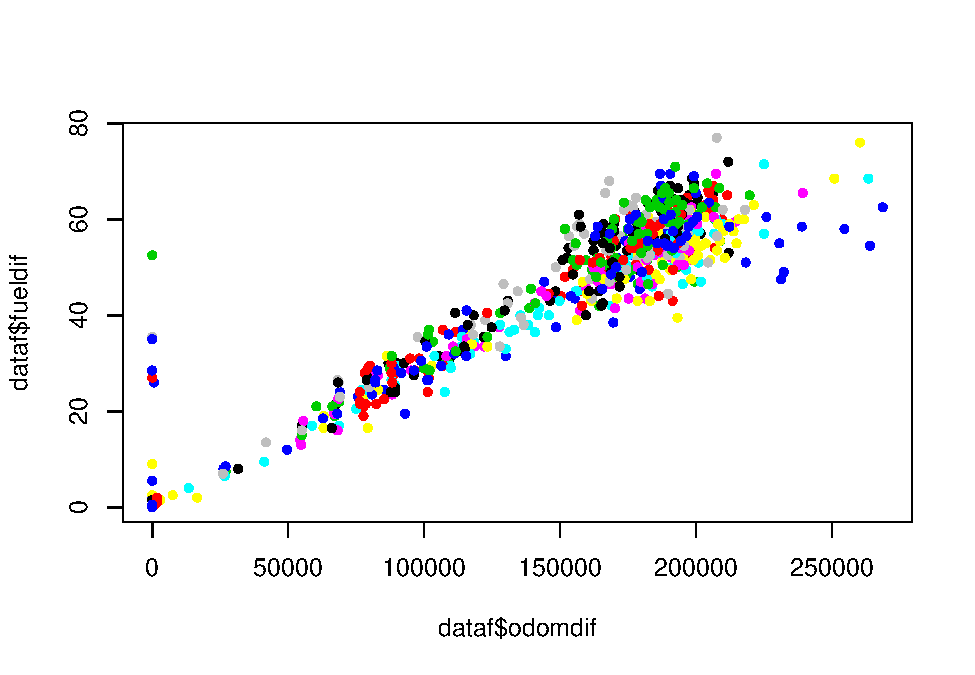
\includegraphics{practica1_files/figure-latex/unnamed-chunk-7-1.pdf}

De donde, tanto en la tabla de ejemplo para el vehículo A1 como en la
gráfica se puede observar la presencia de ruido en los datos.

\section{Deteccíon y Tipificación de datos faltantes y
Outliers.}\label{deteccion-y-tipificacion-de-datos-faltantes-y-outliers.}

\subsection{Deteccíon y Tipificación de datos
faltantes.}\label{deteccion-y-tipificacion-de-datos-faltantes.}

Se creó una variable para tipificar las anomalías que se analizaron.

Primero, se tipificaron los datos que aunque sus valores seguramente son
atípicos, por definición sabemos que no lo son como aquellos en donde
ambos valores (distancia y gasolina) son cero, ya que pueden deberse a
que el vehículo se encuentra parado o aquellos casos en donde se toma
como inicio en la serie de los datos.

Esto mismo pasa en los casos en donde no hubo cambio en el combustible y
por tanto el agrupado de combustible del día se reporta como NA o
aquellos en los que simplemente el dato de gasolina no fue registrado en
todo el día. Estos casos se tipifican como ``Dato faltante gasolina''.

También están los casos en donde no se registra cambio en el odómetro
pero se registra un cambio en la gasolina; esto puede deberse a que las
mediciones de ambas variables no se toman al mismo tiempo y por lo
general los casos se presentan, de hecho, después de un ``descanso'' del
vehículo, es decir una anomalía de tipo ``Vehículo parado'' o una
anomalía de tipo ``Dato faltante gasolina''. Dichos datos se tipifican
como ``Dato inconsistente distancia''.

\begin{Shaded}
\begin{Highlighting}[]
\CommentTok{# No anomalias }
\NormalTok{dataf}\OperatorTok{$}\NormalTok{anomalia<-}\KeywordTok{ifelse}\NormalTok{((dataf}\OperatorTok{$}\NormalTok{fueldif}\OperatorTok{==}\DecValTok{0}\OperatorTok{|}\KeywordTok{is.na}\NormalTok{(dataf}\OperatorTok{$}\NormalTok{fueldif))}\OperatorTok{&}\NormalTok{dataf}\OperatorTok{$}\NormalTok{odomdif}\OperatorTok{==}\DecValTok{0}\NormalTok{,}\StringTok{"Vehículo parado/Inicio"}\NormalTok{,}
                              \KeywordTok{ifelse}\NormalTok{(dataf}\OperatorTok{$}\NormalTok{odomdif}\OperatorTok{==}\DecValTok{0}\OperatorTok{&}\NormalTok{dataf}\OperatorTok{$}\NormalTok{fueldif}\OperatorTok{>}\DecValTok{0}\NormalTok{, }\StringTok{"Dato inconsistente distancia"}\NormalTok{,}
                                     \KeywordTok{ifelse}\NormalTok{(}\KeywordTok{is.na}\NormalTok{(dataf}\OperatorTok{$}\NormalTok{fueldif),}\StringTok{"Dato faltante gasolina"}\NormalTok{,}
                                            \StringTok{"No anomalía"}\NormalTok{)))}
\end{Highlighting}
\end{Shaded}

\subsection{Deteccíon y Tipificación de valores
anomálicos.}\label{deteccion-y-tipificacion-de-valores-anomalicos.}

Se analizaron los datos que resultaron no ser faltantes o anomálicos en
el sentido antes comentado para verificar si existen valores atípicos
los cuales serán descartados del modelaje de predicción.

Se elaboró un boxplot para la variable rendimiento y a partir de ello se
determinaron los valores que son atípicos y se clasificaron como ``Valor
anomálico''.

\begin{Shaded}
\begin{Highlighting}[]
\CommentTok{# Valores anomálicos}

\NormalTok{plo<-dataf[dataf}\OperatorTok{$}\NormalTok{anomalia}\OperatorTok{==}\StringTok{"No anomalía"}\NormalTok{,]}
\NormalTok{bxo<-}\KeywordTok{boxplot}\NormalTok{(plo}\OperatorTok{$}\NormalTok{rendimiento)}
\end{Highlighting}
\end{Shaded}

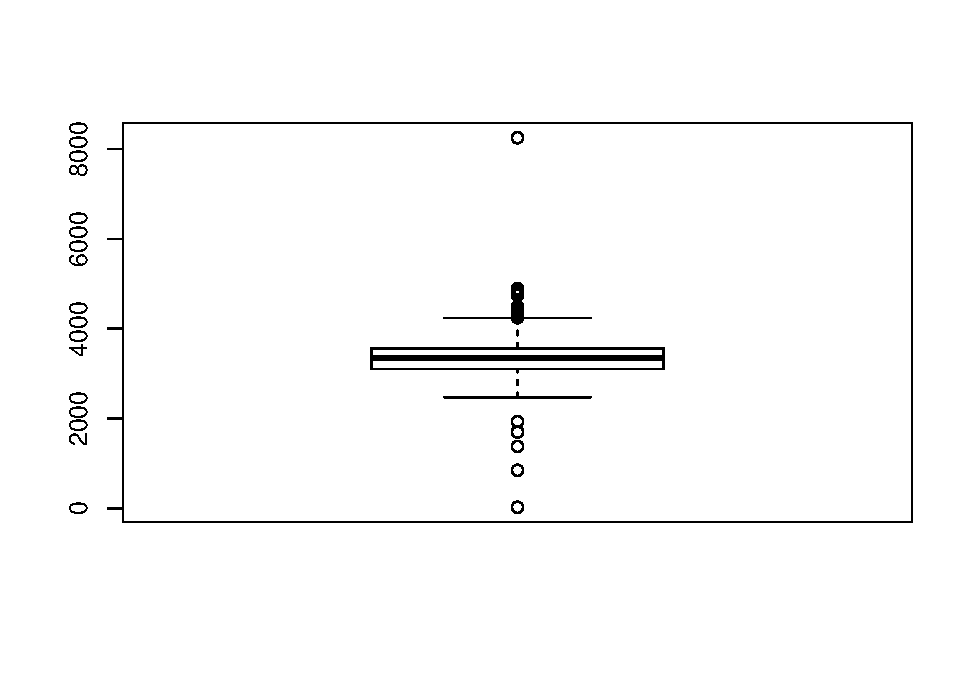
\includegraphics{practica1_files/figure-latex/unnamed-chunk-9-1.pdf}

\begin{Shaded}
\begin{Highlighting}[]
\NormalTok{dataf}\OperatorTok{$}\NormalTok{anomalia<-}\KeywordTok{ifelse}\NormalTok{(dataf}\OperatorTok{$}\NormalTok{rendimiento }\OperatorTok\StringTok{ }\NormalTok{bxo}\OperatorTok{$}\NormalTok{out[bxo}\OperatorTok{$}\NormalTok{out}\OperatorTok{!=}\DecValTok{0}\NormalTok{], }\StringTok{"Valor anomálico"}\NormalTok{,dataf}\OperatorTok{$}\NormalTok{anomalia)}
\NormalTok{dataf}\OperatorTok{$}\NormalTok{anomalia<-}\KeywordTok{as.factor}\NormalTok{(dataf}\OperatorTok{$}\NormalTok{anomalia)}
\end{Highlighting}
\end{Shaded}

La gráfica con los datos anomálicos en rojo (Datos faltantes) y azul
(valores anomálicos) queda:

\begin{Shaded}
\begin{Highlighting}[]
\KeywordTok{plot}\NormalTok{(dataf}\OperatorTok{$}\NormalTok{odomdif, dataf}\OperatorTok{$}\NormalTok{fueldif, }\DataTypeTok{col=}\NormalTok{dataf}\OperatorTok{$}\NormalTok{anomalia, }\DataTypeTok{pch=}\DecValTok{20}\NormalTok{)}
\end{Highlighting}
\end{Shaded}

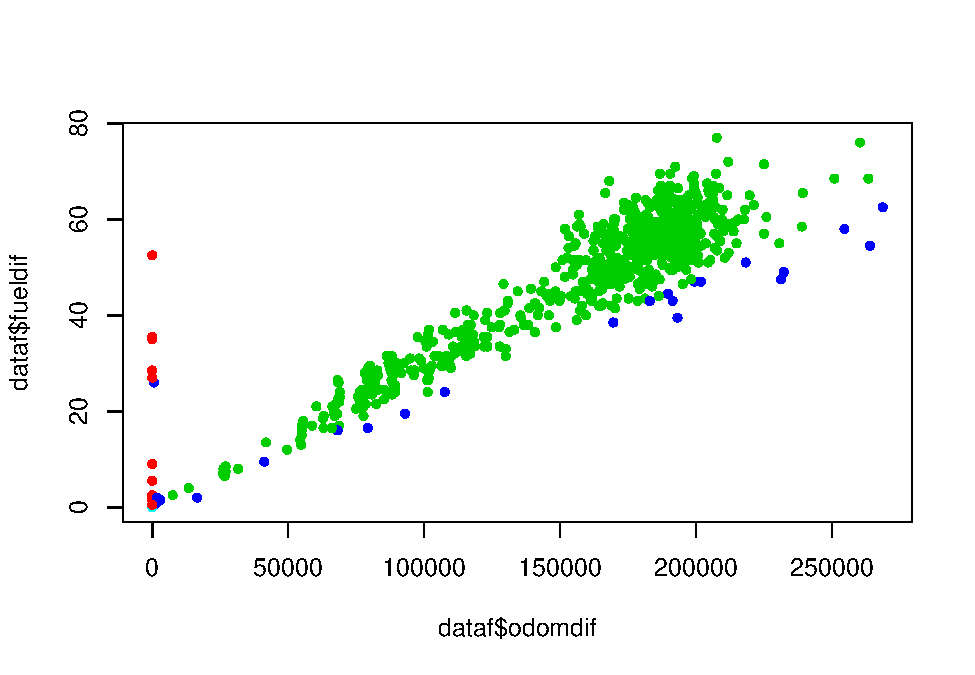
\includegraphics{practica1_files/figure-latex/unnamed-chunk-10-1.pdf}

\subsection{Modelo de regresión}\label{modelo-de-regresion}

Se tomaron todos los datos que no fueran anomalías por datos faltantes o
valores atípicos y se elaboró un modelo de regresión lineal forzando el
intercepto en 0,0 ya que es lógico que con 0 gasolina se recorren 0
unidades de distancia y viceversa análogamente. Se obtienen los
siguientes resultados:

\begin{Shaded}
\begin{Highlighting}[]
\NormalTok{tidy2<-dataf[dataf}\OperatorTok{$}\NormalTok{anomalia}\OperatorTok{==}\StringTok{"No anomalía"}\NormalTok{,]}

\NormalTok{lmod <-}\StringTok{ }\KeywordTok{lm}\NormalTok{(tidy2}\OperatorTok{$}\NormalTok{fueldif }\OperatorTok{~}\StringTok{ }\DecValTok{0}\OperatorTok{+}\StringTok{ }\NormalTok{tidy2}\OperatorTok{$}\NormalTok{odomdif) }
\KeywordTok{summary}\NormalTok{(lmod)}
\end{Highlighting}
\end{Shaded}

\begin{verbatim}
## 
## Call:
## lm(formula = tidy2$fueldif ~ 0 + tidy2$odomdif)
## 
## Residuals:
##      Min       1Q   Median       3Q      Max 
## -14.4144  -2.8814  -0.3086   3.1749  17.4211 
## 
## Coefficients:
##                Estimate Std. Error t value Pr(>|t|)    
## tidy2$odomdif 3.009e-04  1.094e-06   275.1   <2e-16 ***
## ---
## Signif. codes:  0 '***' 0.001 '**' 0.01 '*' 0.05 '.' 0.1 ' ' 1
## 
## Residual standard error: 4.815 on 695 degrees of freedom
## Multiple R-squared:  0.9909, Adjusted R-squared:  0.9909 
## F-statistic: 7.566e+04 on 1 and 695 DF,  p-value: < 2.2e-16
\end{verbatim}

Donde se puede observar que el p-value es muy cercano a 0 y el valor de
la prueba R cuadrada y Rcuadrada ajustada es muy cercano a 1. Nota: Las
demás pruebas estadísticas como lo son la prueba de normalidad de los
residuos, entre otras, salen del alcance de esta práctica.

La gráfica del modelo queda:

\begin{Shaded}
\begin{Highlighting}[]
\KeywordTok{plot}\NormalTok{(tidy2}\OperatorTok{$}\NormalTok{odomdif, tidy2}\OperatorTok{$}\NormalTok{fueldif, }\DataTypeTok{pch=}\DecValTok{20}\NormalTok{)}
\KeywordTok{abline}\NormalTok{(lmod, }\DataTypeTok{lwd=}\DecValTok{2}\NormalTok{, }\DataTypeTok{col=}\StringTok{"blue"}\NormalTok{)}
\end{Highlighting}
\end{Shaded}

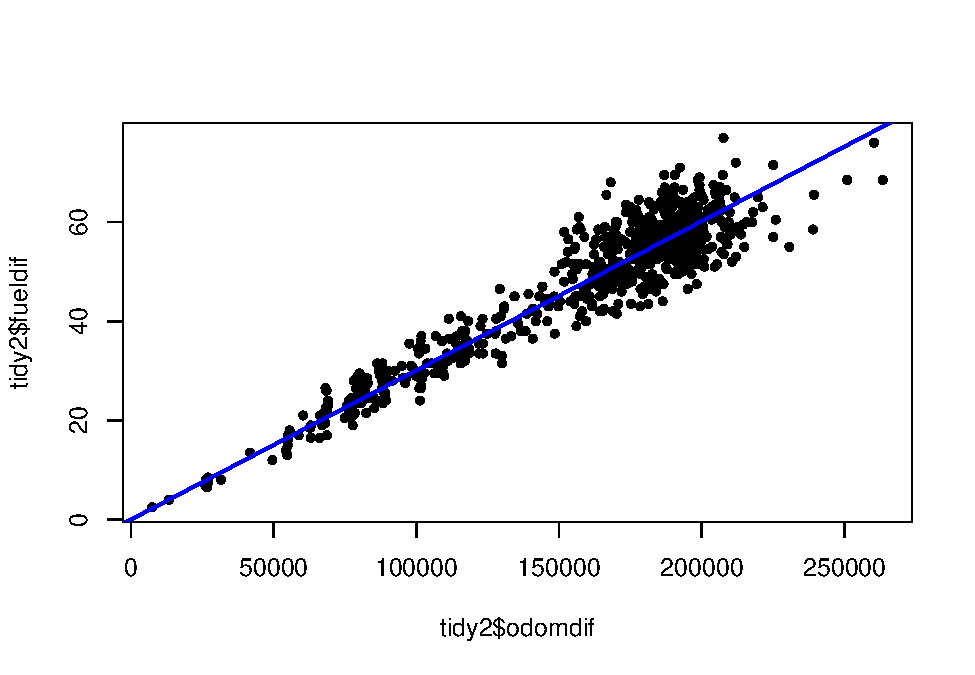
\includegraphics{practica1_files/figure-latex/unnamed-chunk-12-1.pdf}

\subsection{Imputación de valores}\label{imputacion-de-valores}

Si la tabla fuera a ser usada para alguna apllicación y/o reporte diario
de dichas métricas de la flota sería recomendable imputar los valores
faltantes:

\begin{enumerate}
\def\labelenumi{\arabic{enumi}.}
\item
  En los casos en los que el dato del gasolina falta o en los casos en
  que el vehículo estuvo parado, se puede suponer que las mediciones no
  coincidieron y por tanto es mejor estimar de acuerdo a la regresión
  lineal antes hecha.
\item
  En los casos en los que el dato de la distancia es cero pero la
  gasolina no, también se puede asumir que los datos no coincidieron.
\item
  Se calcula de nuevo el rendimiento.
\item
  En el caso de los valores atípicos no se recomienda imputar los
  valores ya que es muy probable que se deba a que el vehículo estuvo en
  tráfico e imputar esos valores sería perder información real.
\end{enumerate}

\begin{Shaded}
\begin{Highlighting}[]
\CommentTok{# Imputación de valores }

\NormalTok{supertidy<-dataf[,}\OperatorTok{-}\KeywordTok{c}\NormalTok{(}\DecValTok{3}\NormalTok{,}\DecValTok{5}\NormalTok{)]}
\NormalTok{supertidy}\OperatorTok{$}\NormalTok{fueldif<-}\KeywordTok{ifelse}\NormalTok{(supertidy}\OperatorTok{$}\NormalTok{anomalia }\OperatorTok\StringTok{ }\KeywordTok{c}\NormalTok{(}\StringTok{"Vehículo parado/Inicio"}\NormalTok{,}\StringTok{"Dato faltante gasolina"}\NormalTok{),}
\NormalTok{                      lmod}\OperatorTok{$}\NormalTok{coefficients[[}\DecValTok{1}\NormalTok{]]}\OperatorTok{*}\NormalTok{supertidy}\OperatorTok{$}\NormalTok{odomdif,}
\NormalTok{                      supertidy}\OperatorTok{$}\NormalTok{fueldif)}
\NormalTok{supertidy}\OperatorTok{$}\NormalTok{odomdif<-}\KeywordTok{ifelse}\NormalTok{(supertidy}\OperatorTok{$}\NormalTok{anomalia }\OperatorTok\StringTok{ }\KeywordTok{c}\NormalTok{(}\StringTok{"Dato inconsistente distancia"}\NormalTok{),}
\NormalTok{                          supertidy}\OperatorTok{$}\NormalTok{fueldif}\OperatorTok{/}\NormalTok{lmod}\OperatorTok{$}\NormalTok{coefficients[[}\DecValTok{1}\NormalTok{]],}
\NormalTok{                          supertidy}\OperatorTok{$}\NormalTok{odomdif)}
\NormalTok{supertidy}\OperatorTok{$}\NormalTok{rendimiento<-supertidy}\OperatorTok{$}\NormalTok{odomdif}\OperatorTok{/}\NormalTok{supertidy}\OperatorTok{$}\NormalTok{fueldif}
\end{Highlighting}
\end{Shaded}

En el ejemplo anterior del vehículo A2 la tabla ``limpia'' con datos
imputados queda:

\begin{Shaded}
\begin{Highlighting}[]
\NormalTok{supertidy[supertidy}\OperatorTok{$}\NormalTok{vehiculo}\OperatorTok{==}\StringTok{"A2"}\NormalTok{,]}
\end{Highlighting}
\end{Shaded}

\begin{verbatim}
##     vehiculo     fecha3   odomdif  fueldif rendimiento
## 429       A2 2018-02-20      0.00  0.00000         NaN
## 430       A2 2018-02-21 109000.00 36.00000    3027.778
## 431       A2 2018-02-22 114200.00 37.00000    3086.486
## 432       A2 2018-02-23 188000.00 64.50000    2914.729
## 433       A2 2018-02-24 190100.00 57.00000    3335.088
## 434       A2 2018-02-25 175200.00 58.00000    3020.690
## 435       A2 2018-02-26 100900.00 33.50000    3011.940
## 436       A2 2018-02-27  98900.00 30.50000    3242.623
## 437       A2 2018-02-28 204700.00 63.50000    3223.622
## 438       A2 2018-03-01 162900.00 56.50000    2883.186
## 439       A2 2018-03-02 199900.00 65.50000    3051.908
## 440       A2 2018-03-03 199200.00 69.00000    2886.957
## 441       A2 2018-03-04 188100.00 65.00000    2893.846
## 442       A2 2018-03-05  80100.00 29.50000    2715.254
## 443       A2 2018-03-06 190900.00 60.00000    3181.667
## 444       A2 2018-03-07 168200.00 57.00000    2950.877
## 445       A2 2018-03-08 193900.00 63.00000    3077.778
## 446       A2 2018-03-09 187100.00 67.00000    2792.537
## 447       A2 2018-03-10 188172.00 64.50000    2917.395
## 448       A2 2018-03-11  98300.00 29.57707    3323.520
## 449       A2 2018-03-12 116323.20 35.00000    3323.520
## 450       A2 2018-03-13  88900.00 29.00000    3065.517
## 451       A2 2018-03-14 188000.00 58.50000    3213.675
## 452       A2 2018-03-15 190600.00 69.50000    2742.446
## 453       A2 2018-03-16 186800.00 69.50000    2687.770
## 454       A2 2018-03-17 175600.00 60.00000    2926.667
## 455       A2 2018-03-18 163800.00 58.50000    2800.000
## 456       A2 2018-03-19 111100.00 32.00000    3471.875
## 457       A2 2018-03-20  27000.00  8.50000    3176.471
## 458       A2 2018-03-21 174000.00 55.50000    3135.135
## 459       A2 2018-03-22 177900.00 61.00000    2916.393
## 460       A2 2018-03-23 115600.00 41.00000    2819.512
## 461       A2 2018-03-24  26200.00  8.00000    3275.000
## 462       A2 2018-03-25      0.00  0.00000         NaN
## 463       A2 2018-03-26   1661.76  0.50000    3323.520
## 464       A2 2018-03-27  49600.00 12.00000    4133.333
## 465       A2 2018-03-28 148500.00 37.50000    3960.000
## 466       A2 2018-03-29 225900.00 60.50000    3733.884
## 467       A2 2018-03-30  80800.00 23.50000    3438.298
##                         anomalia
## 429       Vehículo parado/Inicio
## 430                  No anomalía
## 431                  No anomalía
## 432                  No anomalía
## 433                  No anomalía
## 434                  No anomalía
## 435                  No anomalía
## 436                  No anomalía
## 437                  No anomalía
## 438                  No anomalía
## 439                  No anomalía
## 440                  No anomalía
## 441                  No anomalía
## 442                  No anomalía
## 443                  No anomalía
## 444                  No anomalía
## 445                  No anomalía
## 446                  No anomalía
## 447                  No anomalía
## 448       Dato faltante gasolina
## 449 Dato inconsistente distancia
## 450                  No anomalía
## 451                  No anomalía
## 452                  No anomalía
## 453                  No anomalía
## 454                  No anomalía
## 455                  No anomalía
## 456                  No anomalía
## 457                  No anomalía
## 458                  No anomalía
## 459                  No anomalía
## 460                  No anomalía
## 461                  No anomalía
## 462       Vehículo parado/Inicio
## 463 Dato inconsistente distancia
## 464                  No anomalía
## 465                  No anomalía
## 466                  No anomalía
## 467                  No anomalía
\end{verbatim}

\subsection{Preguntas.}\label{preguntas.}

Nota: Se tomaron los datos limpios, es decir sin considerar anomalías
excepto en el inciso c.

\begin{enumerate}
\def\labelenumi{\alph{enumi}.}
\tightlist
\item
  ¿Qué vehículo da mayor rendimiento?
\end{enumerate}

\begin{Shaded}
\begin{Highlighting}[]
\CommentTok{# vehículo con mayor rendimiento}
\NormalTok{aux<-}\KeywordTok{aggregate}\NormalTok{(plo}\OperatorTok{$}\NormalTok{rendimiento, }\DataTypeTok{by=}\KeywordTok{list}\NormalTok{(plo}\OperatorTok{$}\NormalTok{vehiculo), mean)}
\KeywordTok{colnames}\NormalTok{(aux)<-}\KeywordTok{c}\NormalTok{(}\StringTok{"Vehículo"}\NormalTok{,}\StringTok{"rendimiento_promedio"}\NormalTok{)}
\NormalTok{aux<-aux[}\KeywordTok{order}\NormalTok{(aux}\OperatorTok{$}\NormalTok{rendimiento_promedio, }\DataTypeTok{decreasing=}\NormalTok{T),]}
\NormalTok{aux}
\end{Highlighting}
\end{Shaded}

\begin{verbatim}
##    Vehículo rendimiento_promedio
## 15       A3             3709.865
## 7       A15             3630.158
## 6       A14             3609.469
## 4       A12             3606.524
## 13      A20             3588.235
## 5       A13             3558.640
## 10      A18             3479.436
## 17       A6             3441.529
## 20       A9             3423.880
## 3       A11             3405.619
## 16       A5             3390.432
## 14      A21             3360.189
## 2       A10             3263.025
## 11      A19             3198.678
## 19       A8             3146.800
## 12       A2             3109.128
## 18       A7             3107.599
## 9       A17             3096.768
## 1        A1             3076.492
## 8       A16             3012.026
\end{verbatim}

\begin{enumerate}
\def\labelenumi{\alph{enumi}.}
\setcounter{enumi}{1}
\tightlist
\item
  ¿Qué vehículo trabajó mas días?
\end{enumerate}

\begin{Shaded}
\begin{Highlighting}[]
\CommentTok{# Vehículo que trabajó más días}
\NormalTok{aux<-}\KeywordTok{aggregate}\NormalTok{(plo}\OperatorTok{$}\NormalTok{fecha3, }\DataTypeTok{by=}\KeywordTok{list}\NormalTok{(plo}\OperatorTok{$}\NormalTok{vehiculo), min)}
\KeywordTok{colnames}\NormalTok{(aux)<-}\KeywordTok{c}\NormalTok{(}\StringTok{"Vehículo"}\NormalTok{,}\StringTok{"min"}\NormalTok{)}
\NormalTok{aux2<-}\KeywordTok{aggregate}\NormalTok{(plo}\OperatorTok{$}\NormalTok{fecha3, }\DataTypeTok{by=}\KeywordTok{list}\NormalTok{(plo}\OperatorTok{$}\NormalTok{vehiculo), max)}
\KeywordTok{colnames}\NormalTok{(aux2)<-}\KeywordTok{c}\NormalTok{(}\StringTok{"Vehículo"}\NormalTok{,}\StringTok{"max"}\NormalTok{)}
\NormalTok{aux3<-}\KeywordTok{merge}\NormalTok{(aux, aux2, }\DataTypeTok{by=}\StringTok{"Vehículo"}\NormalTok{)}
\NormalTok{aux3}\OperatorTok{$}\NormalTok{dif<-aux3}\OperatorTok{$}\NormalTok{max}\OperatorTok{-}\NormalTok{aux3}\OperatorTok{$}\NormalTok{min}
\NormalTok{aux3<-aux3[}\KeywordTok{order}\NormalTok{(aux3}\OperatorTok{$}\NormalTok{dif, }\DataTypeTok{decreasing=}\NormalTok{T),]}
\NormalTok{aux3}
\end{Highlighting}
\end{Shaded}

\begin{verbatim}
##    Vehículo        min        max     dif
## 7       A15 2018-02-21 2018-03-31 38 days
## 11      A19 2018-02-21 2018-03-31 38 days
## 2       A10 2018-02-22 2018-03-31 37 days
## 3       A11 2018-02-22 2018-03-31 37 days
## 4       A12 2018-02-22 2018-03-31 37 days
## 5       A13 2018-02-22 2018-03-31 37 days
## 6       A14 2018-02-22 2018-03-31 37 days
## 8       A16 2018-02-22 2018-03-31 37 days
## 9       A17 2018-02-21 2018-03-30 37 days
## 12       A2 2018-02-21 2018-03-30 37 days
## 13      A20 2018-02-21 2018-03-30 37 days
## 14      A21 2018-02-22 2018-03-31 37 days
## 15       A3 2018-02-22 2018-03-31 37 days
## 16       A5 2018-02-22 2018-03-31 37 days
## 17       A6 2018-02-21 2018-03-30 37 days
## 18       A7 2018-02-22 2018-03-31 37 days
## 19       A8 2018-02-22 2018-03-30 36 days
## 20       A9 2018-02-22 2018-03-30 36 days
## 1        A1 2018-02-21 2018-03-28 35 days
## 10      A18 2018-02-22 2018-03-29 35 days
\end{verbatim}

\begin{enumerate}
\def\labelenumi{\alph{enumi}.}
\setcounter{enumi}{2}
\tightlist
\item
  ¿Cuál es el combustible total utilizado por la flota por semana?
\end{enumerate}

\begin{Shaded}
\begin{Highlighting}[]
\CommentTok{# Combustible total de la flota por semana}

\KeywordTok{library}\NormalTok{(lubridate)}
\end{Highlighting}
\end{Shaded}

\begin{verbatim}
## 
## Attaching package: 'lubridate'
\end{verbatim}

\begin{verbatim}
## The following object is masked from 'package:base':
## 
##     date
\end{verbatim}

\begin{Shaded}
\begin{Highlighting}[]
\NormalTok{aux<-fuel}
\NormalTok{aux}\OperatorTok{$}\NormalTok{semana<-}\KeywordTok{week}\NormalTok{(}\KeywordTok{ymd}\NormalTok{(}\KeywordTok{as.character}\NormalTok{(aux}\OperatorTok{$}\NormalTok{fecha3)))}

\NormalTok{totalv<-}\KeywordTok{aggregate}\NormalTok{(aux}\OperatorTok{$}\NormalTok{valor, }\DataTypeTok{by=}\KeywordTok{list}\NormalTok{(aux}\OperatorTok{$}\NormalTok{vehiculo, aux}\OperatorTok{$}\NormalTok{semana), min)}
\KeywordTok{colnames}\NormalTok{(totalv)<-}\KeywordTok{c}\NormalTok{(}\StringTok{"v"}\NormalTok{,}\StringTok{"s"}\NormalTok{,}\StringTok{"min"}\NormalTok{)}
\NormalTok{aux2<-}\KeywordTok{aggregate}\NormalTok{(aux}\OperatorTok{$}\NormalTok{valor, }\DataTypeTok{by=}\KeywordTok{list}\NormalTok{(aux}\OperatorTok{$}\NormalTok{vehiculo, aux}\OperatorTok{$}\NormalTok{semana), max)}
\KeywordTok{colnames}\NormalTok{(aux2)<-}\KeywordTok{c}\NormalTok{(}\StringTok{"v"}\NormalTok{,}\StringTok{"s"}\NormalTok{,}\StringTok{"max"}\NormalTok{)}
\NormalTok{totalv<-}\KeywordTok{merge}\NormalTok{(totalv, aux2, }\DataTypeTok{by=}\KeywordTok{c}\NormalTok{(}\StringTok{"v"}\NormalTok{,}\StringTok{"s"}\NormalTok{))}
\NormalTok{totalv}\OperatorTok{$}\NormalTok{dif<-totalv}\OperatorTok{$}\NormalTok{max}\OperatorTok{-}\NormalTok{totalv}\OperatorTok{$}\NormalTok{min}

\NormalTok{totalf<-}\KeywordTok{aggregate}\NormalTok{(totalv}\OperatorTok{$}\NormalTok{dif, }\DataTypeTok{by=}\KeywordTok{list}\NormalTok{(totalv}\OperatorTok{$}\NormalTok{s), sum)}
\KeywordTok{colnames}\NormalTok{(totalf)<-}\KeywordTok{c}\NormalTok{(}\StringTok{"Semana"}\NormalTok{,}\StringTok{"Total_gasolina"}\NormalTok{)}
\NormalTok{totalf}
\end{Highlighting}
\end{Shaded}

\begin{verbatim}
##   Semana Total_gasolina
## 1      8         4651.5
## 2      9         6647.0
## 3     10         6589.0
## 4     11         6586.5
## 5     12         5964.0
## 6     13         4315.0
\end{verbatim}

\begin{enumerate}
\def\labelenumi{\alph{enumi}.}
\setcounter{enumi}{3}
\tightlist
\item
  ¿Cuál es la correlación entre ambas variables (distancia,
  combustible)? Correlación de Pearson:
\end{enumerate}

\begin{Shaded}
\begin{Highlighting}[]
\KeywordTok{cor}\NormalTok{(plo}\OperatorTok{$}\NormalTok{odomdif, plo}\OperatorTok{$}\NormalTok{fueldif)}
\end{Highlighting}
\end{Shaded}

\begin{verbatim}
## [1] 0.9278223
\end{verbatim}


\end{document}
